% Un document standard de type article
% 
% Rédigé pour les étudiants de sciences de la Terre de l'Université de Lyon par
% Laurent Pouilloux, Yanick Ricard, Stéphane Labrosse, Frédéric Chambat
%
% Licence Creative Commons
% Attribution-NonCommercial-ShareAlike 3.0 Unported (CC BY-NC-SA 3.0) 
%
 
\documentclass[10pt]{article}

%\Declareunicodecharacter{2009}{\,}
%% PACKAGES
% Regles typographiques francaises
\usepackage[french]{babel}
% Utilisation des accents et d'un encodage standard (UTF8)
\usepackage[utf8]{inputenc}
\usepackage[T1]{fontenc}
% Chargement d'une police
\usepackage[scaled]{helvet}
\renewcommand*\familydefault{\sfdefault}
% Dimensions de la page
\usepackage{a4wide}
% Creation des liens hypertextes dans le document
\usepackage[colorlinks=true, breaklinks=true, linkcolor=black, citecolor=blue,]{hyperref}
% Definition des entetes de pages
\usepackage{fancyhdr}
\pagestyle{fancyplain}
% Utilisation d'images
\usepackage{graphicx}
% Utilisation de tableaux evolues
\usepackage{tabularx}
% Commandes pour les URL et email
\usepackage{url}
% Pour faire des exemples d'utilisation de commandes LaTeX
\usepackage{example}
% Gestion avancee de la bibliographie
%\usepackage[]{natbib}
% Les couleurs
\usepackage{color}
\usepackage{cite}
\usepackage{geometry}
\geometry{
 a4paper,
 total={170mm,257mm},
 left=20mm,
 top=20mm,
 }
\usepackage{hhline}
\usepackage{multicol}
\usepackage{multirow}
\usepackage{booktabs}
\usepackage[colorlinks=true, breaklinks=true, linkcolor=black, citecolor=blue,]{hyperref}

%% COMMANDES
% Profondeur de la table des matieres
%\setcounter{tocdepth}{2}
% Agrandissement de la zone reservee aux entetes
%\addtolength{\headheight}{1.5pt}
% Definitions de commandes pour mettre en couleur
%\def\R#1{\textcolor{red}{#1}}
%\def\B#1{\textcolor{blue}{#1}}
%

\bibliographystyle{unsrt}
\begin{document}

% Informations concernant le document
\title{Describing the movement behavior of \textit{Chelonoidis chilensis}}
\author{The turtle team}

\date{september 2021}
% Page de titre automatique
\maketitle
% Resume du document

\section*{Introduction}

The Charco turtle (\textit{Chelonoidis chilensis}) lives in the region of San Antonio del Oeste on the east coast of Argentina. They live in a dry biome constistuted of weeds and arbusts named el monte. They are endangered because of the destruction of their natural habitat by extensive cattle breeding, but also because they are illegaly taken as pets. They actively participate to the functionnig of their ecosystem by dispersing the seeds they eat but also because their eggs are eaten by small predators and scavengers. Unfortunately little quantitative study has been made on their movement which makes difficult its conservation. It is said that these turtles are more mobile in spring during the reproductive season, especially males. In this study, we measured the daily home range (maximum distance traveled in one day) of charco turtles in different period of the year and of different sex. 

\section*{Material}

We went on the same location 3 times: in march 2020, in november 2021 and in january 2021. In march 2020, only one female was followed with a device containing a GPS. In november 2020, 5 males and 7 females were followed. In january 2021, 1 male and 3 females were followed which makes in total 6 males and 11 females. The positions were obtained with two methods : with a GPS or with a yagui antenna.

Moreover, in november 2020, 7 turtles have been followed with a spool and line technique.

\section*{Results}

\subsection*{Home range}

We plotted the trajectories of each turtle (Supplementary Material). Point (0,0) corresponds to the position of the turtle at the beginning of the first day of measure. We removed all the points which would imply that the speed of the turtle is above 1km/h as they are likely to be artefacts. Each color corresponds to a different day in the season. Some points with the GPS were taken with regular interval of time 5 minutes or 10 minutes, allowing us to evaluate the speed of the turtle at these different intervals of time (Figure ~\ref{fig:speed}). We can see that the mode of the distribution is 1 m/min using the 5 minute intervals, but is lower using the 10 minutes interval. This is excpected because the turtle have more time to change its direction and thus bias our perception of its speed.

\begin{figure}[!ht]
\centering
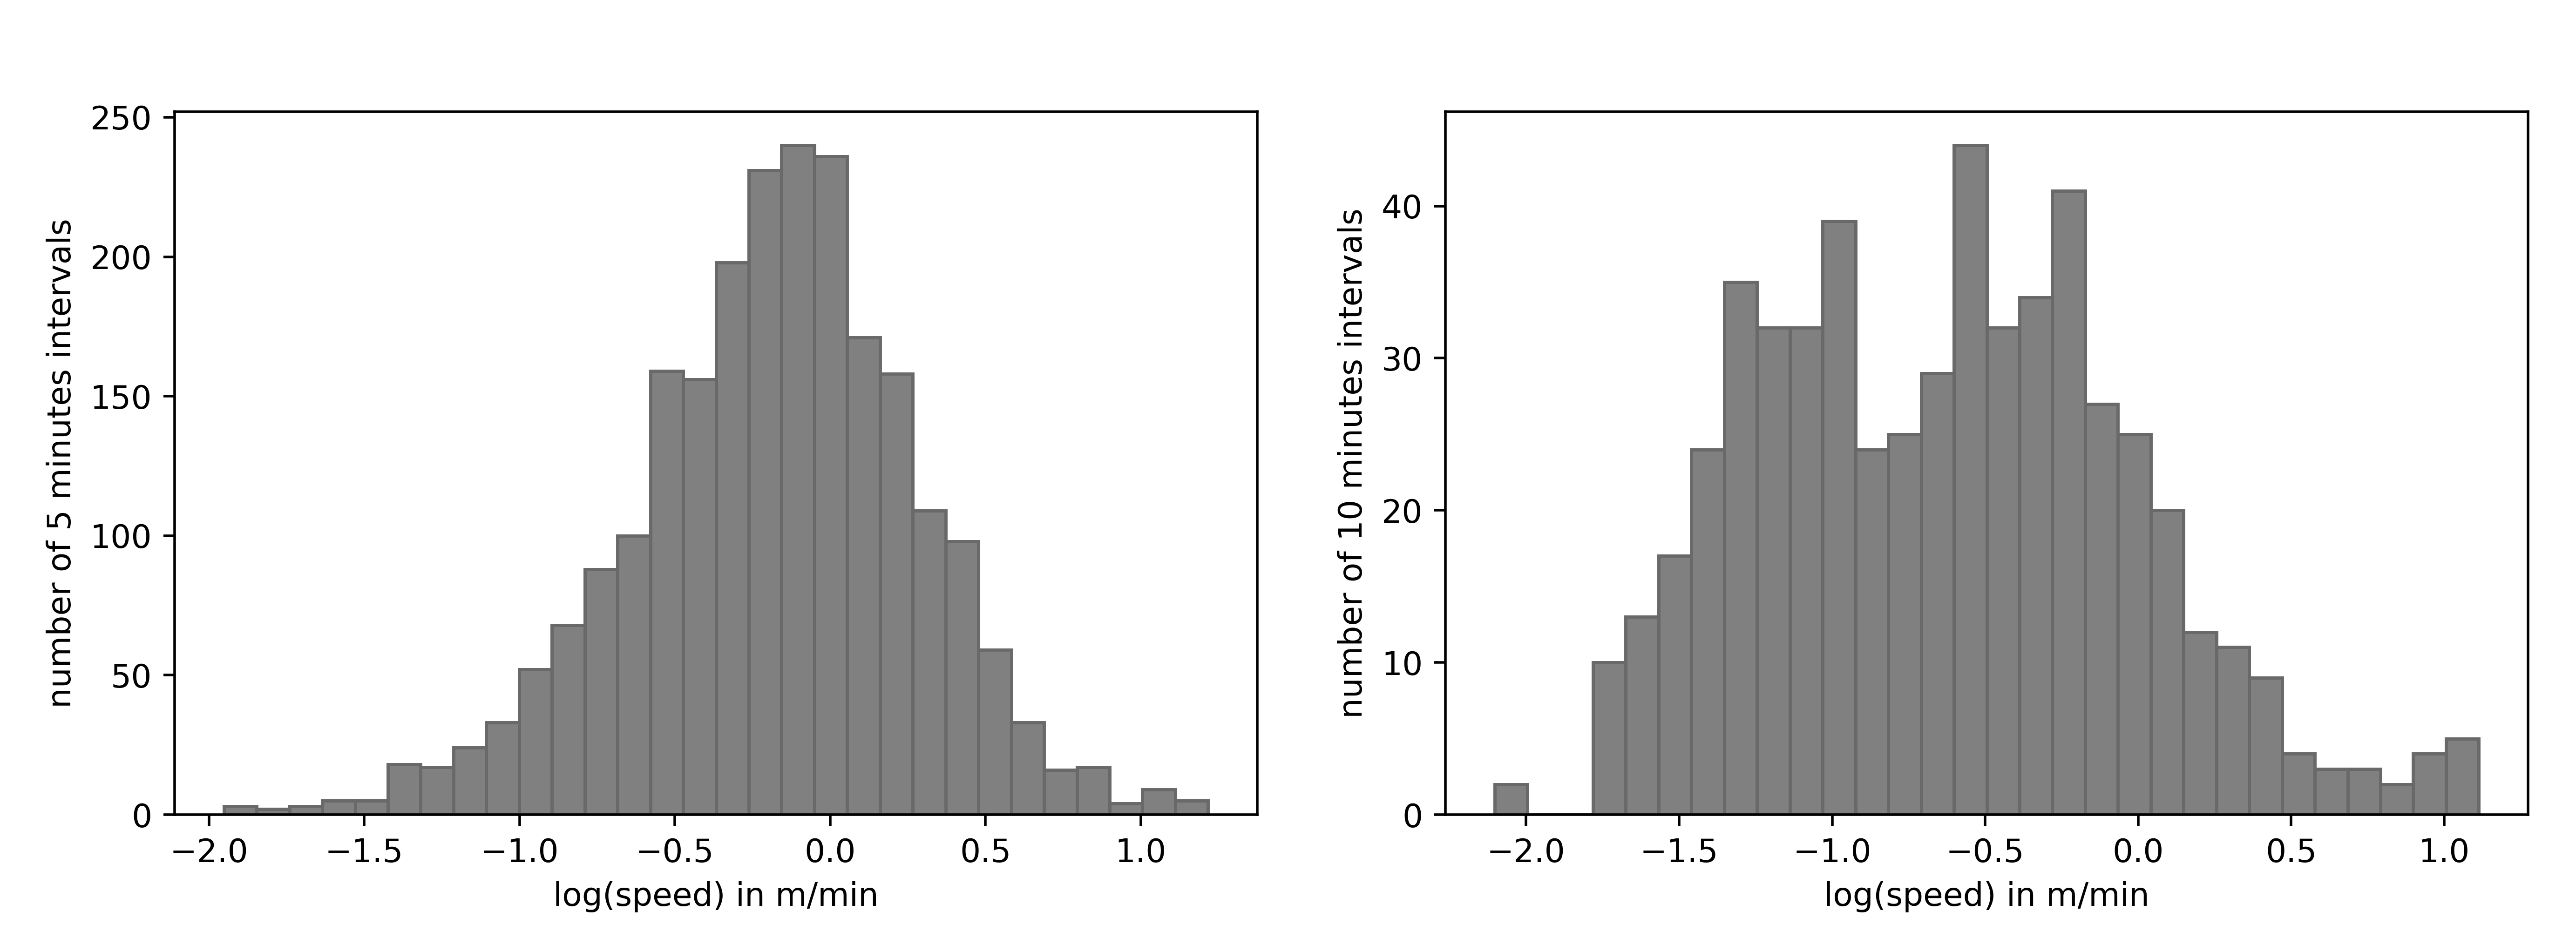
\includegraphics[width=0.9\columnwidth]{speed_distribution_5m.png}
\caption{Distribution of speed of the turtles measured on intervals of 5 minutes (left) or 10 minutes (right).}
\label{fig:speed}
\end{figure}

We plotted the positions of all the turtles depending on the period of the year (Figure ~\ref{fig:sexo} left). This time, point (0,0) corresponds to the position of the turtle at the beginning of the day in order to visualize how much does a turtle can disperse during one day (Figure ~\ref{fig:temporada} left). We did the same but distinguishing between sexes rather than season (Figure ~\ref{fig:sexo} left).

\begin{figure}[!ht]
\centering
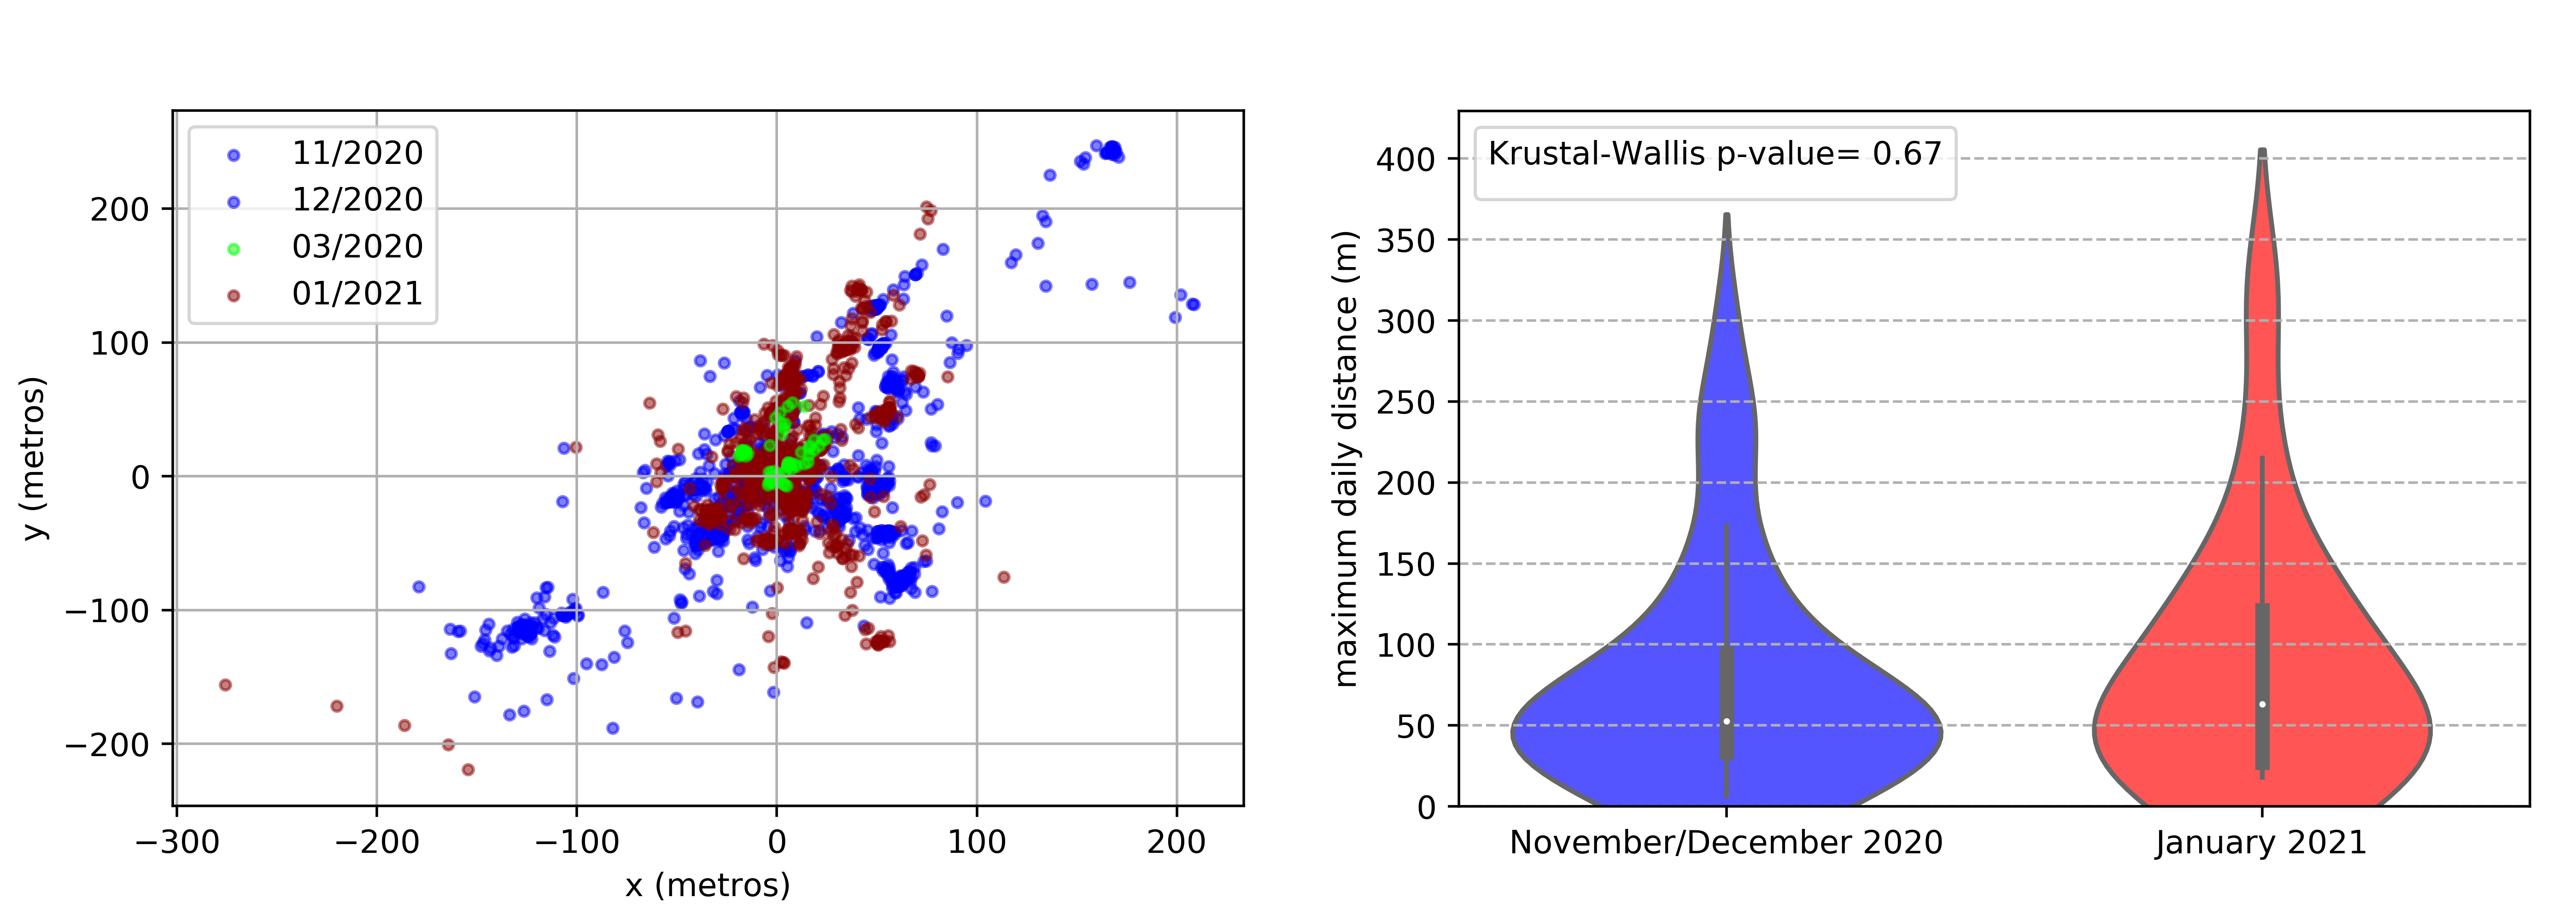
\includegraphics[width=0.9\columnwidth]{all_turtles_temporada.png}
\caption{Left - Positions of the turtles estimated with all methods. For each turtle, point (0,0) corresponds to the position at the begining of the day. In blue are the positions during november/december, in red the positions in january, and in green the positions in march. Right - Distribution of the maximum distance from the starting point for each turtle and for each day. In blue during november/december and in red during january. In march, only one turtle was followed on 2 days so we did not include this measure in our comparison of distribution (we can hardly make a distribution out of 2 points).}
\label{fig:temporada}
\end{figure}

Then, for each day and for each turtle, we computed the maximal distance from the starting point. We distinguished once again the different seasons (Figure ~\ref{fig:temporada} right) and sexes (Figure ~\ref{fig:sexo} right). We can see that the mean is around 50 m but the variability is great. Indeed, the dispersion can reach more than 300 meters. There are few days from which we can measure maximal distance, and thus the distributions to compare have a small number of data. Then, we used the non-parametric test of Krustal-Wallis to determine if the distribution of daily dispersions are the same between seasons and sexes. We can see that the distributions cannot be told appart since the p-values are larger than 0.05. In march, only one turtle was followed on 2 days so we did not include this measure in our comparison of distribution.


\begin{figure}[!ht]
\centering
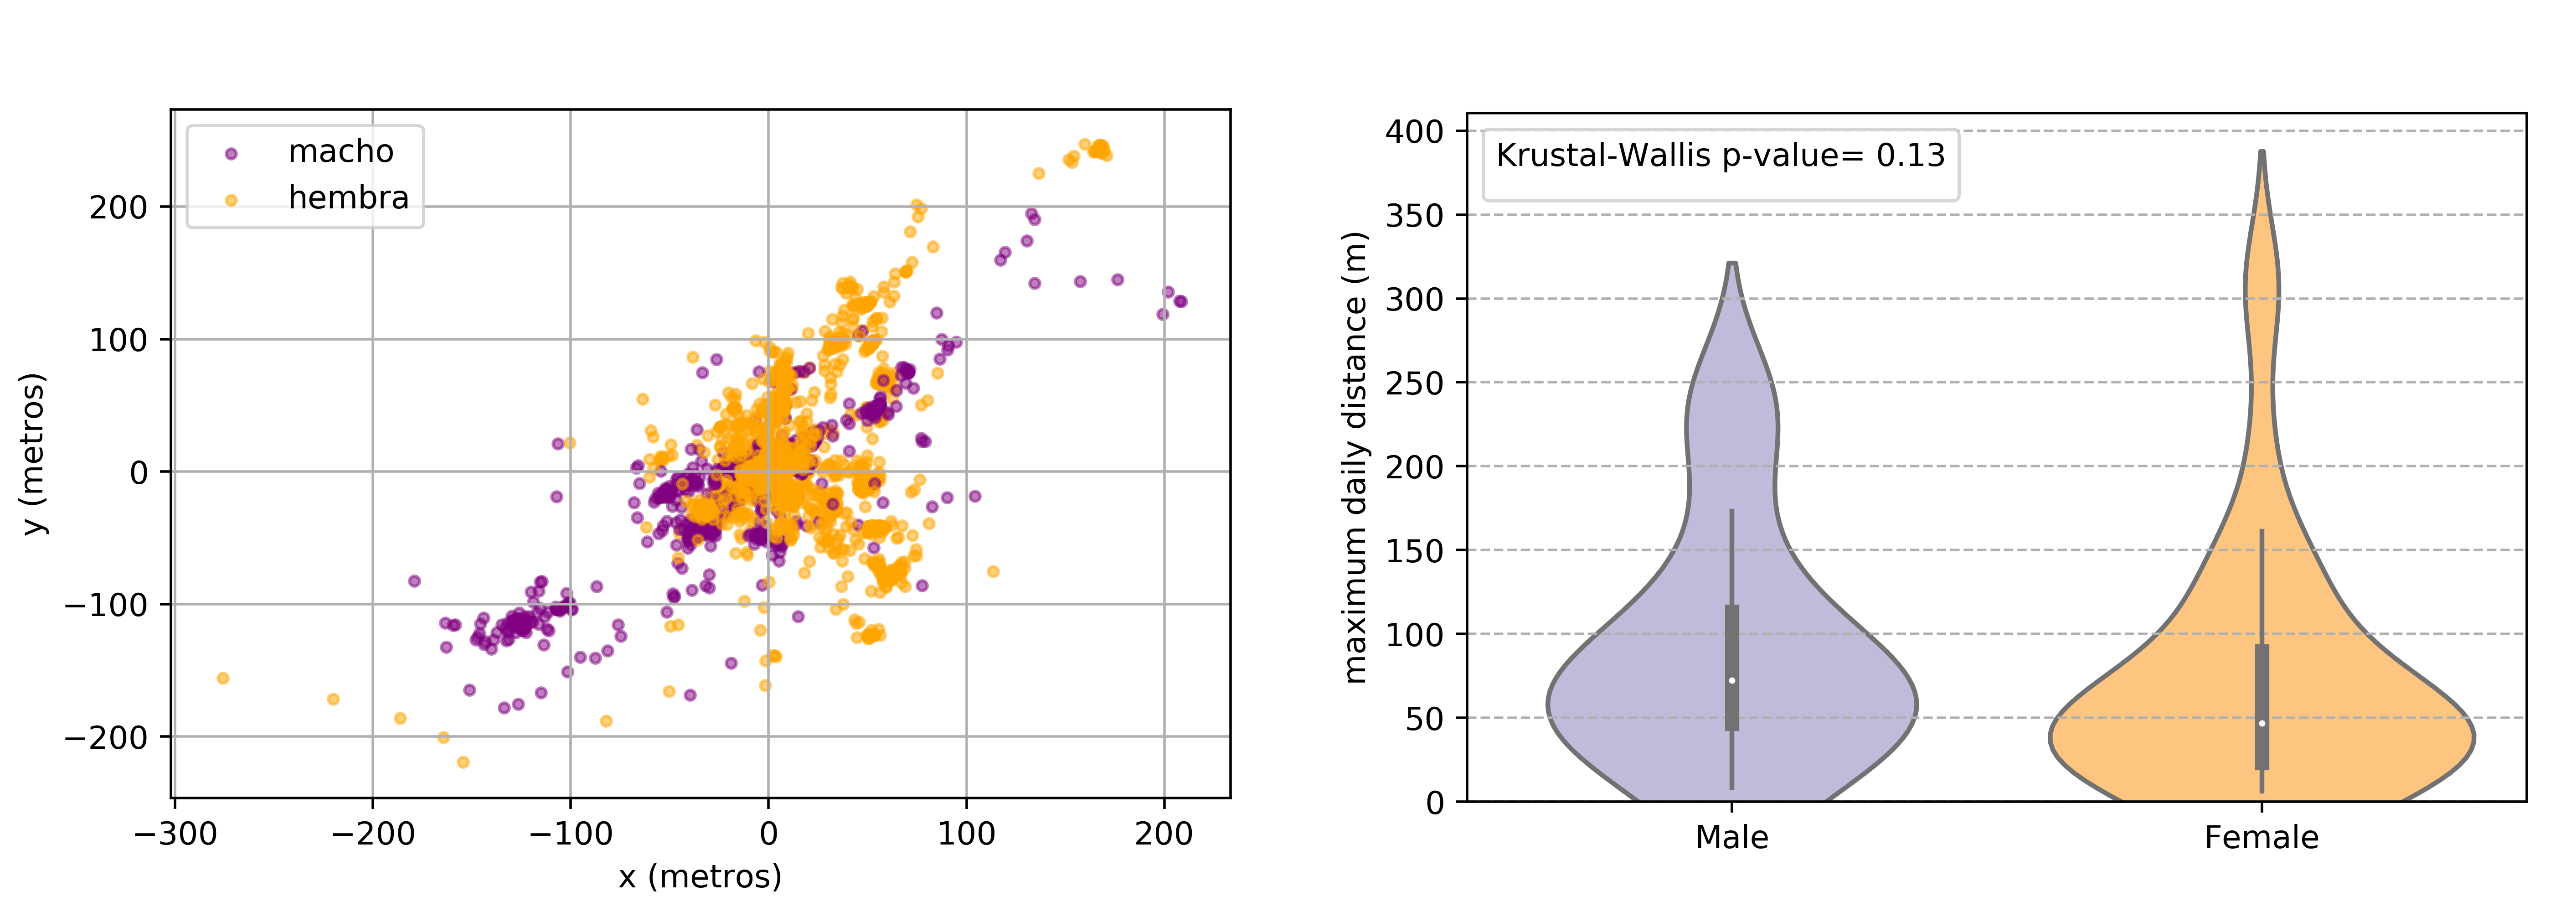
\includegraphics[width=0.9\columnwidth]{all_turtles_sexo.png}
\caption{Left - Positions of the turtles estimated with all methods. For each turtle, point (0,0) corresponds to the position at the begining of the day. In yellow are the positions of the females, and in purple the positions of the males. Right - Distribution of the maximum distance from the starting point for each turtle and for each day. In yellow for the females and in purple for the males.}
\label{fig:sexo}
\end{figure}

\subsection*{Movement description}

Trajectories measured with GPS have the advantage to include a temporal dimension with little error on the animal location. However, the little deviation of the position due to the imprecisions of the device doesn't allow us to measure correctly the distribution of turning angles.

On the other hand, trajectories assessed with spool and line technique have a much finer spatial resolution than GPS tracking. It allows us to compute the distribution of turning angles without these artefacts.

We measured all turning angles for the trajectories of 7 turtles followed with spool and line technique between november and december 2020 ~\ref{fig:angles}. We can see that most angles show little deviation from the direct line which can indicate that the turtle knows more or less where it is going.

\begin{figure}[!ht]
\centering
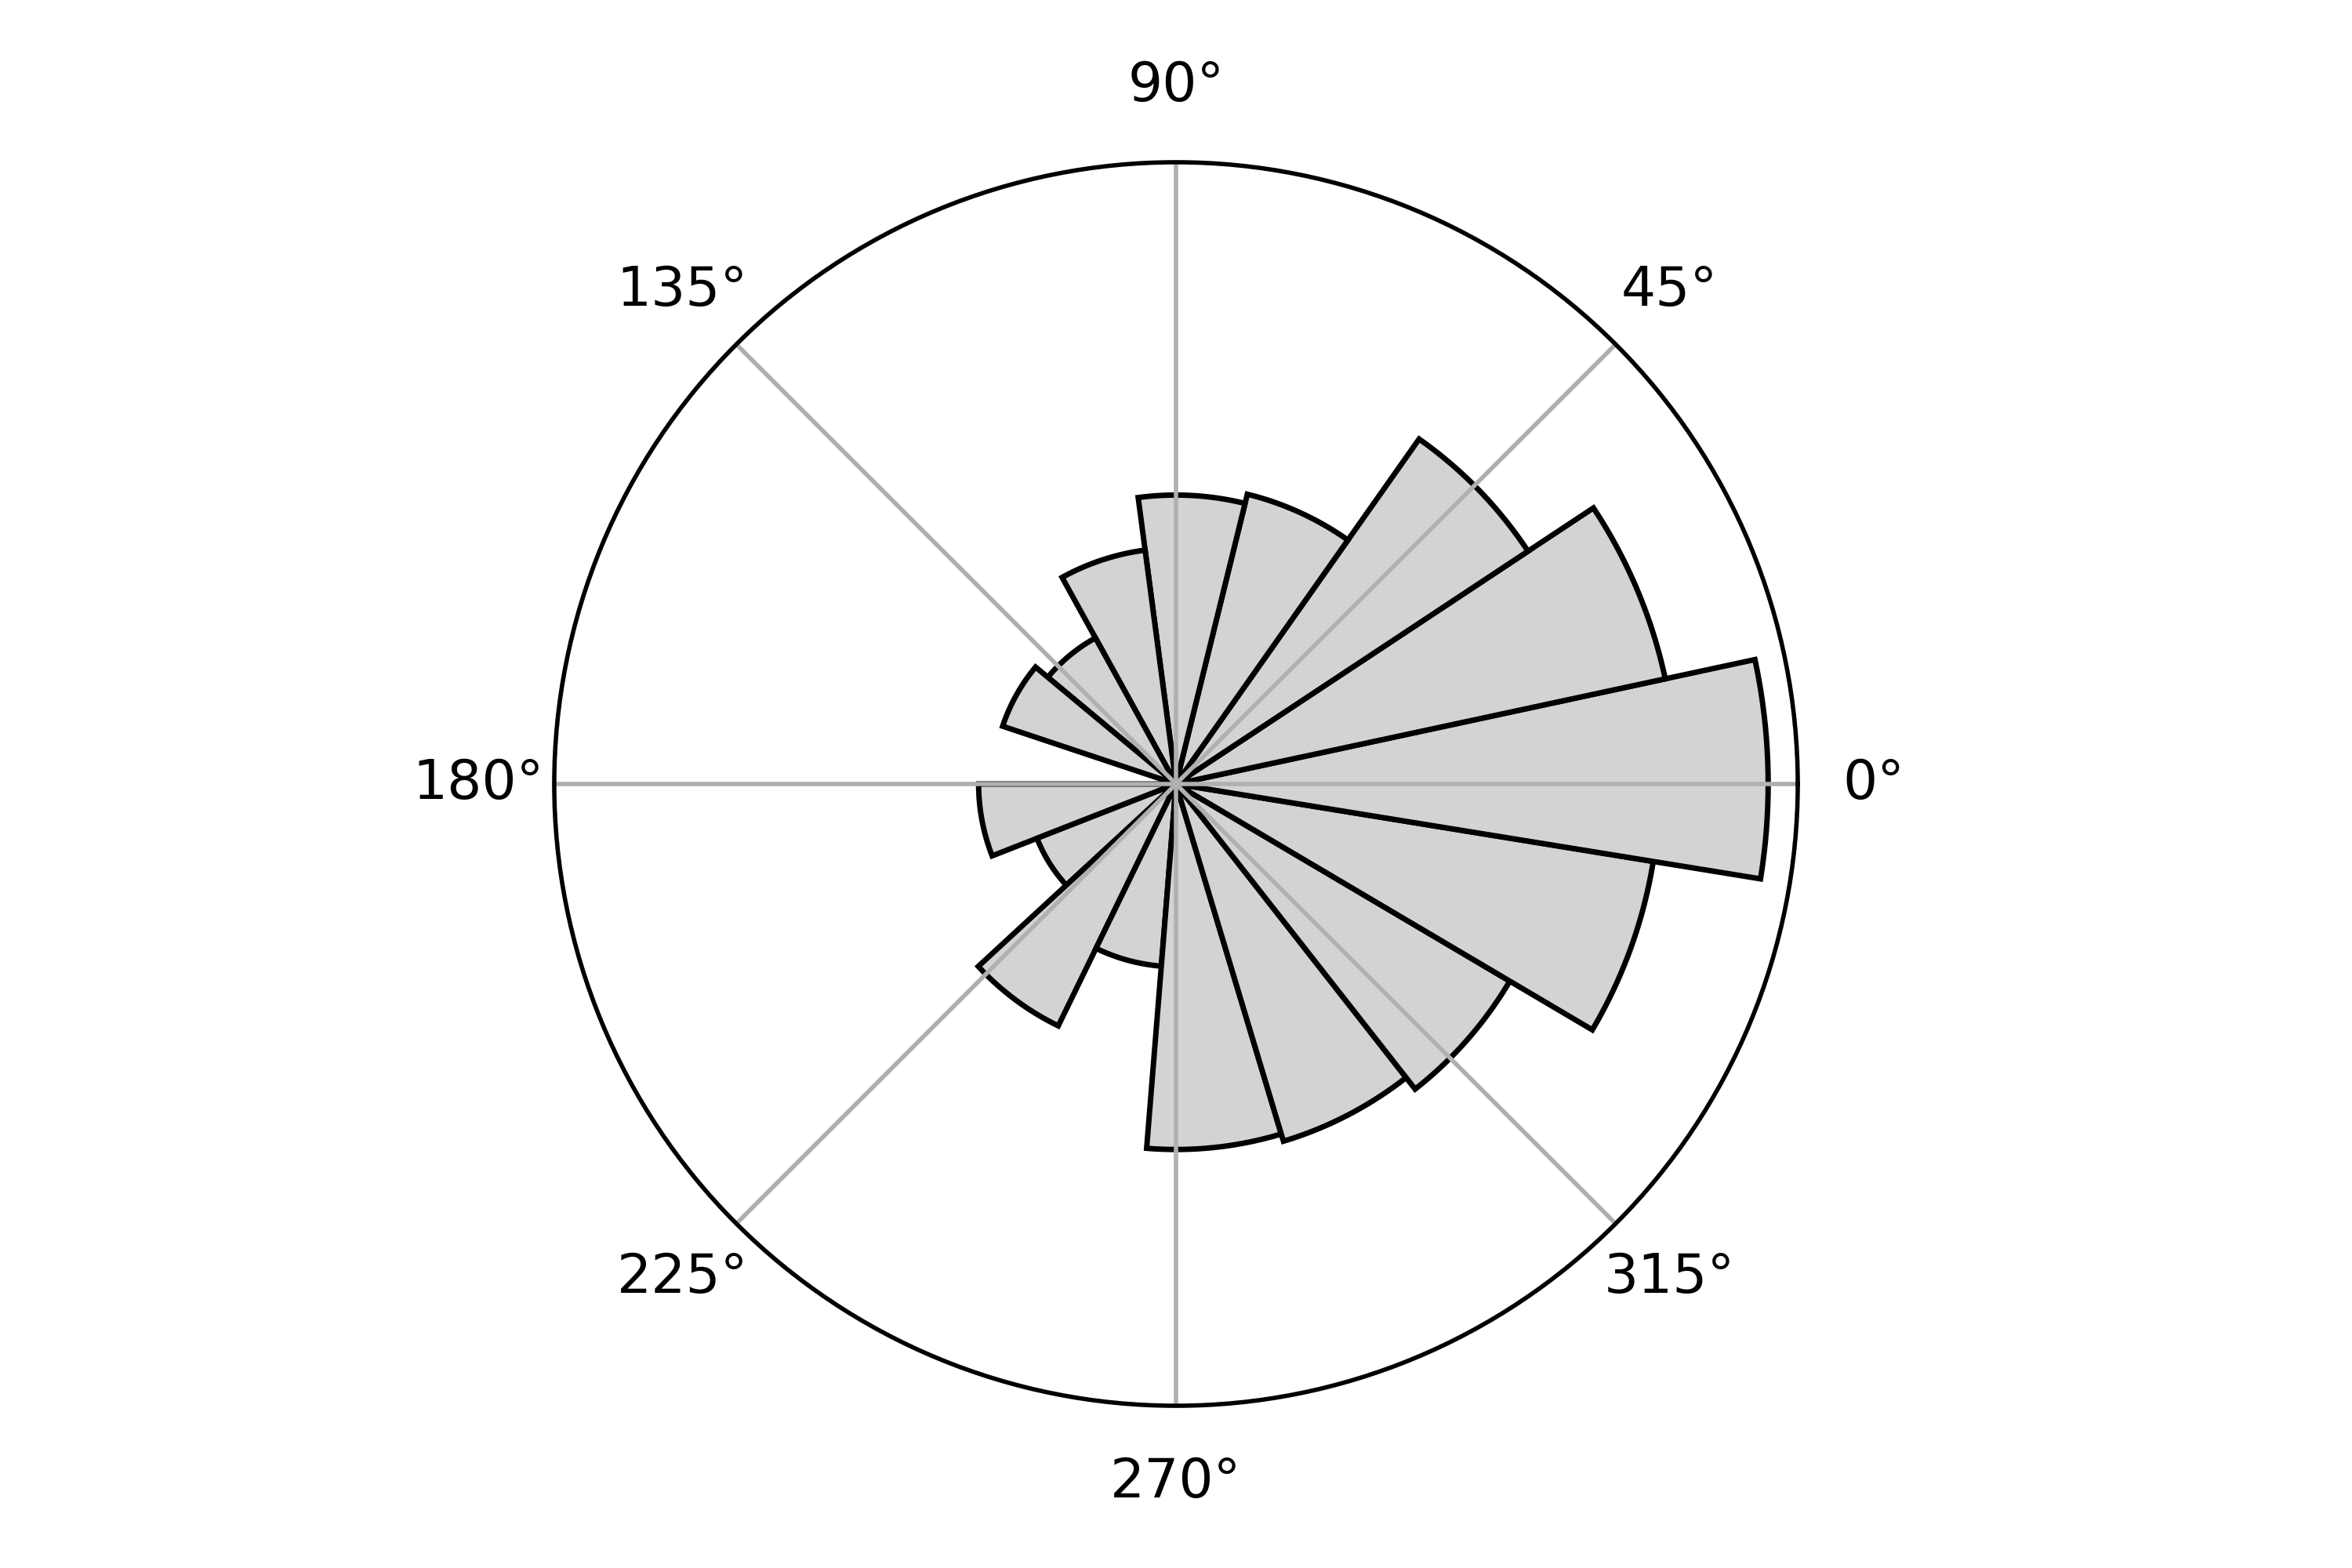
\includegraphics[width=0.9\columnwidth]{radial_histograms.png}
\caption{Distribution of 340 turning angles measured on 7 turtles tracked with spool and line technique between november and december 2020. The radius of the circle corresponds to around 25\% of the turning angles }
\label{fig:angles}
\end{figure}

\section*{Discussion}

We showed that the turtles move at a speed of around 1m/min. This means that in a 5 minutes interval they move in average at 5 meters. This distance is within the error of the GPS, consequently that we cannot distinguish a movement from a GPS error at this timescale. Two options can be explored. The first one is to take intervals with more time taking the risk to underestimate the actual speed of the animal. The second one is to couple the data to accelerometry in order to distinguish periods of inactivity from period where the turtle is in movement.

The daily dispersion of the turtle is not that much affected by this problem. However, the measures on few turtles and on few days do not allow us to distinguish the dispersion between sexes and seasons.

We showed that turtles move mostly forward with little deviation from the straight line but measurement of mean square deviation when the turtle is active would allow us to better determine the movement behavior of the animal.


\end{document}
